\section{Metodologia}
\label{sec:metodologia}

O estudo foi conduzido de ponta a ponta, do planejamento dos objetivos de nível de serviço (SLOs) à coleta e interpretação dos experimentos. O enfoque é aplicado e experimental: toda a instrumentação foi construída diretamente no repositório ValorizeAI, o que permite a reprodução dos resultados.

\subsection{Tipo de Pesquisa e Estratégia Geral}

O trabalho caracteriza-se como uma \textbf{pesquisa aplicada} conduzida como \textbf{estudo de caso} de um sistema real em produção. A estratégia seguiu quatro fases iterativas. No \textbf{planejamento}, foram definidos os SLOs (latência P95 de 300~ms, erro $<$0{,}5\%, disponibilidade $\geq$99{,}5\%), mapeadas as cotas vigentes do Cloud Run (10 instâncias de 1~vCPU / 1~GiB, totalizando 10 vCPU) e estimado como essa limitação poderia afetar o throughput máximo almejado, o que orientou as cargas aplicadas. Em seguida veio a \textbf{preparação do ambiente}: módulos Terraform provisionaram rede, bancos e serviços gerenciados; Docker Compose reproduziu localmente PostgreSQL, Redis e a stack de observabilidade; o Makefile encapsulou tarefas de lint, testes e execução dos cenários. Na etapa de \textbf{execução controlada}, os cenários k6 de leitura e leitura/escrita foram disparados contra a API em Cloud Run enquanto o pipeline assíncrono recebia um lote adicional de tarefas no Cloud Tasks, exercitando os workers HTTP. Por fim, na \textbf{coleta e análise}, as métricas agregadas (latência, throughput, taxa de erro) foram extraídas dos CSVs e painéis do Cloud Monitoring, e as observações qualitativas sobre o teste de filas foram registradas juntamente com o tempo total de drenagem, subsidiando os capítulos de implementação e resultados.

\subsection{Arquitetura do Ambiente Experimental}

A Figura \ref{fig:arquitetura} sintetiza os componentes usados nos experimentos. O tráfego HTTP/HTTPS entra por um \textbf{Cloud Load Balancer} com \textbf{Cloud CDN}, que reduz a latência de \textit{assets} estáticos e protege o backend com inspeção WAF. Esse tráfego é encaminhado para dois serviços Cloud Run:
\begin{itemize}
    \item \textbf{API Laravel}: processa requisições REST, expõe endpoints usados pelos testes k6 e orquestra o pipeline assíncrono.
    \item \textbf{Laravel Reverb}: mantém conexões WebSocket persistentes para eventos em tempo real; é tratado como serviço independente para permitir escalonamento específico.
\end{itemize}

Ambos os serviços acessam o \textbf{Memorystore for Redis}, usado simultaneamente como cache de leitura (padrão \textit{cache-aside}) e como \textit{backplane} Pub/Sub do Reverb. O armazenamento transacional permanece no \textbf{Cloud SQL for PostgreSQL}, que atende às operações de leitura e escrita executadas durante os testes. Para workloads assíncronos, a API publica tarefas em \textbf{Cloud Tasks}, que aciona workers HTTP também hospedados no Cloud Run. Diferentemente de filas baseadas em \textit{polling}, o Cloud Tasks opera no modo \textit{push}: quando novas tarefas são registradas, o serviço dispara requisições para os endpoints configurados e o Cloud Run instancia containers apenas enquanto houver demanda. Isso elimina processos \textit{long living} dedicados a escutar filas e garante elasticidade automática durante rajadas. Artefatos grandes (extratos e relatórios) são persistidos no \textbf{Cloud Storage}, mas não fizeram parte dos testes de carga.

Para refletir o ambiente em produção, o Cloud SQL foi configurado como instância personalizada \emph{db-perf-optimized-N-2} (2~vCPU e 16~GiB de RAM), garantindo buffers suficientes para os planos complexos das consultas analíticas sem alterar o perfil de custos do sistema.

\begin{figure}[ht]
    \centering
    \resizebox{\linewidth}{!}{%
    \begin{tikzpicture}[node distance=1.5cm, every node/.style={font=\footnotesize, align=center}]
        \node (cdn) [draw, rounded corners, fill=gray!15, minimum width=5cm, minimum height=0.9cm] {Cloud Load Balancer + Cloud CDN};
        \node (api) [draw, rounded corners, fill=blue!10, minimum width=3cm, minimum height=0.9cm, below left=1.1cm and 2.0cm of cdn] {Cloud Run\\API};
        \node (reverb) [draw, rounded corners, fill=blue!10, minimum width=3cm, minimum height=0.9cm, below=1.1cm of cdn] {Cloud Run\\Reverb};
        \node (workers) [draw, rounded corners, fill=blue!10, minimum width=3cm, minimum height=0.9cm, below right=1.1cm and 2.0cm of cdn] {Cloud Run\\Workers};
        \node (shared) [draw, rounded corners, fill=orange!15, minimum width=6cm, minimum height=1.2cm, below=1.3cm of reverb] {Cloud SQL + Memorystore (Redis) + Cloud Storage};
        \node (tasks) [draw, rounded corners, fill=green!10, minimum width=5cm, minimum height=0.9cm, below=1.0cm of shared] {Cloud Tasks};

        \draw[->, thick] (cdn) -- (api);
        \draw[->, thick] (cdn) -- (reverb);
        \draw[->, thick] (cdn) -- (workers);
        \draw[->, thick] (api) -- (shared);
        \draw[->, thick] (reverb) -- (shared);
        \draw[->, thick] (workers) -- (shared);
        \draw[->, thick] (api) |- (tasks);
        \draw[->, thick] (tasks) -| (workers);
    \end{tikzpicture}}
    \caption{Arquitetura utilizada nos experimentos.}
    \label{fig:arquitetura}
\end{figure}

\subsection{Desenvolvimento da Aplicação e Modelo de Dados}

O desenvolvimento do ValorizeAI avançou em paralelo à infraestrutura. O \textit{backend} Laravel concentra o domínio financeiro (contas, orçamentos, categorizações) e expõe APIs REST e eventos WebSocket consumidos pelo painel React. Essa base inclui ingestão automática de extratos (OFX/CSV), reconciliação assistida por filas, categorização por embeddings e automações que propagam atualizações de saldo e metas em tempo real. Os 	extit{workers} HTTP são os responsáveis por processar os pipelines mais caros (importação de transações, geração de relatórios, envio de notificações) e publicam eventos para o Reverb, fechando o ciclo com a interface.

O modelo relacional, sintetizado na Figura \ref{fig:modelo-dados}, reflete os invariantes do domínio multi-inquilino. Usuários controlam múltiplas contas vinculadas a bancos e moedas distintas, cada conta agrega transações com divisão por categorias, e os orçamentos mensais impõem limites e alocações que retroalimentam o painel de metas. Camadas de auditoria (logs de importação, feedback de categorização e embeddings vetoriais em pgvector) conectam a coleta de dados com os recursos de IA usados para sugerir classificações.

\begin{figure}[ht]
    \centering
    \resizebox{0.95\linewidth}{!}{%
    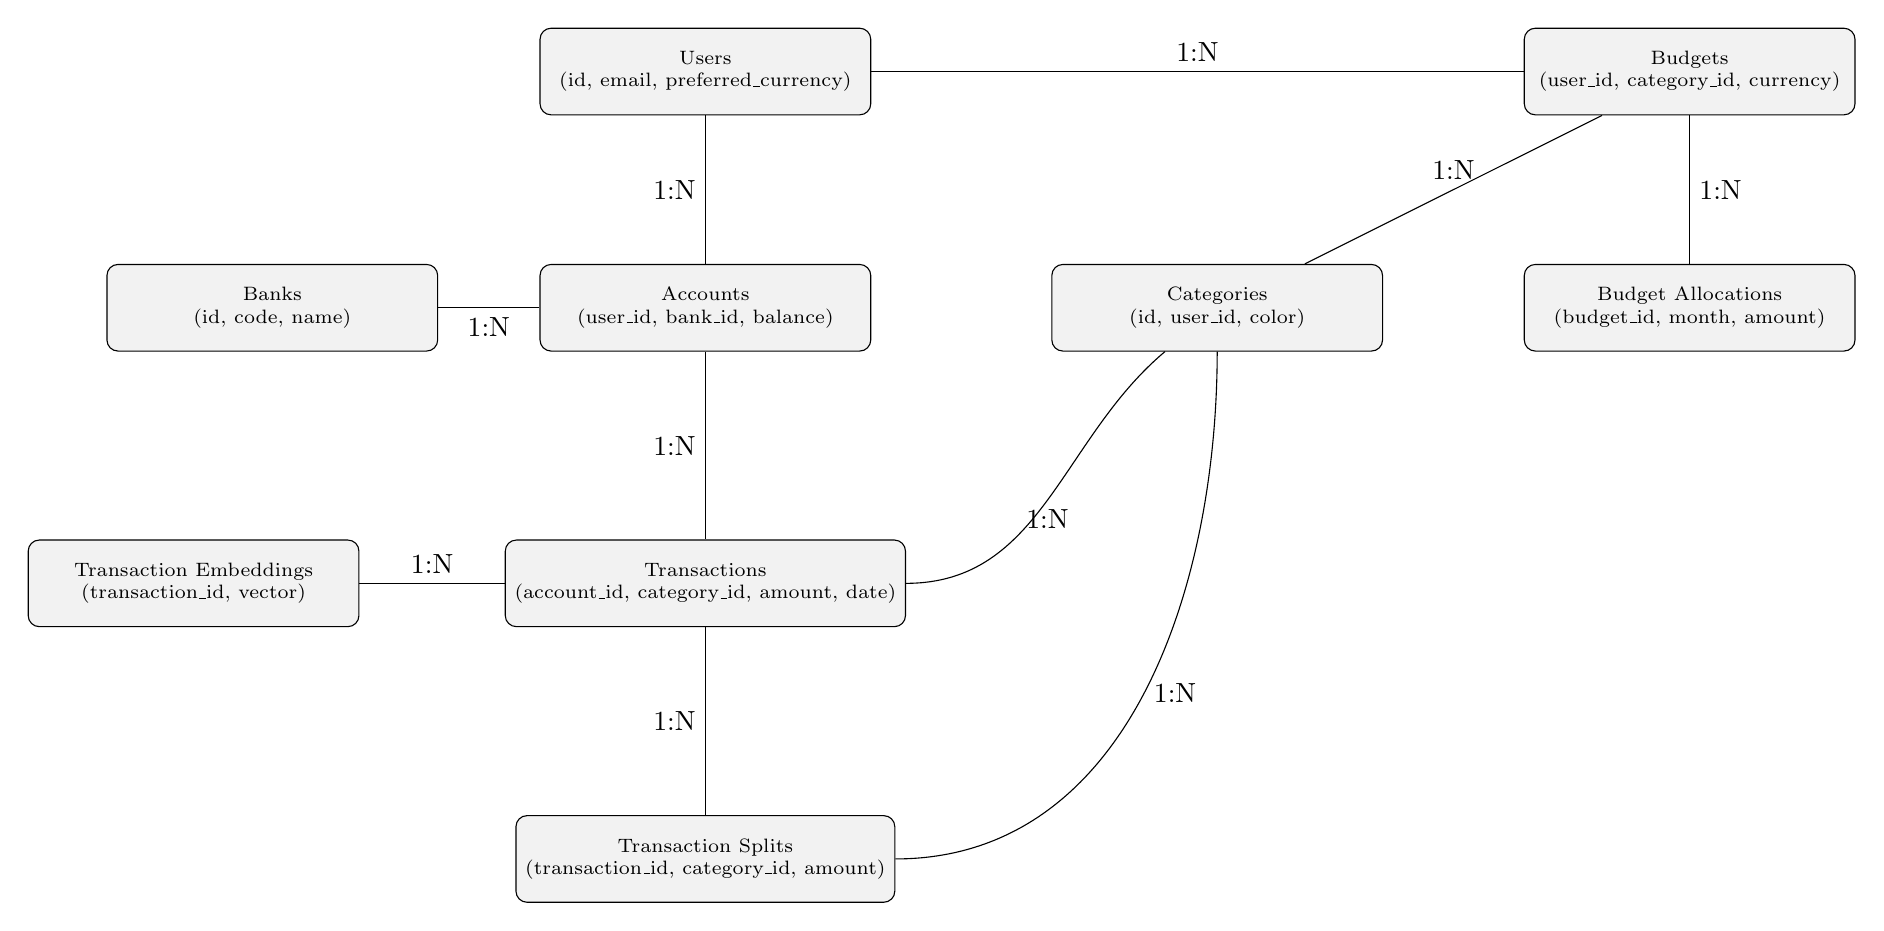
\begin{tikzpicture}[
        table/.style={draw, rounded corners, fill=gray!10, minimum width=4.2cm, minimum height=1.1cm, font=\scriptsize, align=center},
        every edge/.style={->, very thick, >=Stealth}
    ]
        \node (users) at (0,1.5) [table] {Users\\(id, email, preferred\_currency)};
        \node (banks) at (-5.5,-1.5) [table] {Banks\\(id, code, name)};
        \node (accounts) at (0,-1.5) [table] {Accounts\\(user\_id, bank\_id, balance)};
        \node (transactions) at (0,-5.0) [table] {Transactions\\(account\_id, category\_id, amount, date)};
        \node (splits) at (0,-8.5) [table] {Transaction Splits\\(transaction\_id, category\_id, amount)};

        \node (categories) at (6.5,-1.5) [table] {Categories\\(id, user\_id, color)};
        \node (embeddings) at (-6.5,-5.0) [table] {Transaction Embeddings\\(transaction\_id, vector)};
        \node (budgets) at (12.5,1.5) [table] {Budgets\\(user\_id, category\_id, currency)};
        \node (allocations) at (12.5,-1.5) [table] {Budget Allocations\\(budget\_id, month, amount)};

        \draw (users) -- node[midway,left]{1:N} (accounts);
        \draw (banks) -- node[midway,below]{1:N} (accounts);
        \draw (accounts) -- node[midway,left]{1:N} (transactions);
        \draw (transactions) -- node[midway,left]{1:N} (splits);
        \draw (transactions) -- node[midway,above]{1:N} (embeddings);

        \draw (users) -- node[midway,above]{1:N} (budgets);
        \draw (categories) -- node[midway,above]{1:N} (budgets);
        \draw (budgets) -- node[midway,right]{1:N} (allocations);

        \draw (categories) to[out=-140,in=0] node[midway,below]{1:N} (transactions);
        \draw (categories) to[out=-90,in=0] node[midway,right]{1:N} (splits);
    \end{tikzpicture}}
    \caption{Modelo lógico central derivado do esquema relacional do ValorizeAI.}
    \label{fig:modelo-dados}
\end{figure}

\subsection{Ferramentas e Processo de Preparação}

Do ponto de vista de engenharia, três pilares garantiram a reprodutibilidade:
\textbf{(i)} \emph{Infraestrutura como Código}: os módulos Terraform descrevem VPC, balanceadores, Cloud Run, Cloud SQL, Redis e Cloud Tasks. Cada mudança passa por \textit{plan/apply} versionado, evitando deriva de ambiente.
\textbf{(ii) Ambientes determinísticos}: o Makefile e os manifestos Docker recompõem o stack local (PostgreSQL, Redis e PHP 8.4) idêntico ao ambiente de teste antes de qualquer execução k6.
\textbf{(iii) Observabilidade}: o Cloud Monitoring consolidou métricas de latência, uso de CPU/memória e backlog das filas. A adoção de OpenTelemetry e Loki/Tempo permanece como trabalho futuro.

A camada de infraestrutura como código segue um arranjo modular: cada elemento da arquitetura (Cloud SQL, Memorystore, Cloud Run, Cloud Tasks e o balanceador com CDN) é definido como módulo independente e parametrizado com as mesmas variáveis de projeto, região e rótulos. Esses módulos expõem \textit{outputs} que encadeiam os serviços — por exemplo, o endereço privado do banco é injetado na definição do serviço Cloud Run, e o host/porta do Redis alimenta tanto a API quanto o servidor de WebSockets. A malha também contempla recursos de suporte, como a VPC dedicada ao tráfego serverless, a conexão ao Service Networking para disponibilizar IPs privados e os segredos no Secret Manager (credenciais de banco, tokens de API, chaves de serviço). Dependências explícitas garantem que os segredos e o emparelhamento de rede estejam prontos antes do provimento dos contêineres, evitando condições de corrida. Como resultado, o ambiente completo pode ser criado, atualizado ou destruído com um único \textit{apply}, assegurando rastreabilidade das mudanças de infraestrutura no mesmo repositório do código-fonte.

\subsection{Planejamento dos SLOs e Desenho dos Cenários}

Com base nas premissas de negócio e na literatura de SRE \cite{mccoy_slo_2020,google_sre_book_main}, o sistema foi avaliado contra três metas: latência P95 $\leq 300$~ms, taxa de erro $<$ 0{,}5\% e disponibilidade mensal $\geq 99{,}5\%$. A cota vigente do Cloud Run (10 instâncias de 1~vCPU/1~GiB) limita o total de CPU disponível; no nosso cenário isso significou que os testes deveriam aumentar a carga até consumir essas 10 vCPU — ambos os cenários chegaram ao teto de 10 instâncias ativas, permitindo documentar o comportamento imediatamente antes do esgotamento.

Dois cenários foram modelados:
\begin{enumerate}
    \item \textbf{Leitura intensiva}: 1{.}000 usuários virtuais consultando listas de transações por 17 minutos em seis estágios, exercitando cache Redis + réplica de leitura do PostgreSQL.
    \item \textbf{Mistura leitura/escrita}: 650 usuários virtuais alternando consultas e criação de transações durante 21 minutos, forçando locks no banco e pressionando o pipeline de escrita.
\end{enumerate}
Além desses ensaios HTTP, foi planejado um \textbf{teste de filas} no qual um volume elevado de tarefas artificiais percorre o fluxo Cloud Tasks → workers HTTP, permitindo observar o tempo de drenagem e a elasticidade dos consumidores assíncronos.

O roteiro de leitura replica o padrão de navegação predominante no produto: cada VU monta filtros distintos para o endpoint \texttt{GET /api/transactions}, alternando entre contas e categorias, e mantém um \textit{think time} de 1~s para simular o tempo de leitura na interface. As etapas de carga (150→1000 VUs) formam uma curva contínua que aquece a cache, sustenta o platô de 600–900 VUs e aplica um pico curto de 1.000 VUs apenas para identificar o ponto de saturação com todas as instâncias do Cloud Run ativas.

O roteiro misto introduz um endpoint de provisionamento que entrega um token e dados exclusivos para cada VU, impedindo que múltimos usuários escrevam na mesma conta. O fluxo executa leituras em 65\% das iterações, \texttt{POST /api/transactions} em 20\% e \texttt{GET /api/accounts} no restante, com cargas crescendo até 650 VUs. Esse percentual reproduz a relação leitura/escrita observada nos logs reais, enquanto o estágio final concentra o esforço em operações que seguram locks no PostgreSQL.

Para o ensaio assíncrono, um script independente publica 51{,}58~mil tarefas em lotes para o Cloud Tasks. Cada inserção ativa automaticamente os workers HTTP no Cloud Run, que escalam horizontalmente conforme o backlog. As métricas coletadas (vazão em tarefas/min e tempo de drenagem) servem para validar o comportamento da arquitetura orientada a eventos.

\subsection{Execução dos Experimentos}

Cada rodada segue os passos:
\begin{enumerate}
    \item \textbf{Preparação dos dados}: seeds e factories povoam o PostgreSQL com contas, transações e orçamentos realistas; a instância Redis é pre-aquecida com métricas e dashboards frequentes.
    \item \textbf{Disparo do cenário}: os perfis do k6 focados em leitura e no mix leitura/escrita são executados via Makefile, apontando para o domínio público do Cloud Load Balancer; estágios, VUs e SLIs monitorados seguem o planejamento experimental.
    \item \textbf{Registro automático}: os resultados agregados são gravados em CSVs (latência, taxa de erro, uso de VUs) e correlacionados com as métricas de infraestrutura capturadas pelo Cloud Monitoring.
    \item \textbf{Teste de filas}: um script HTTP produz um lote adicional de tarefas e a drenagem é acompanhada por meio das métricas do Cloud Tasks e dos logs dos workers.
\end{enumerate}

\subsection{Coleta e Integração das Evidências}

As evidências produzidas sustentam as análises de arquitetura, implementação e resultados:
\begin{itemize}
    \item \textbf{Planilhas de latência e throughput}: derivadas dos CSVs exportados pelo k6, utilizadas posteriormente para comparar as métricas observadas com os SLOs.
    \item \textbf{Series temporais de infraestrutura}: capturas dos dashboards do Cloud Monitoring registram uso de CPU das instâncias Cloud Run, saturação do Redis e backlog do Cloud Tasks durante cada rodada.
    \item \textbf{Relatos de execução}: cada rodada é registrada em um diário experimental com horários, parâmetros e observações qualitativas sobre o comportamento do sistema.
\end{itemize}

Essa metodologia garante rastreabilidade completa entre arquitetura, implementação e resultados, pois cada passo experimental está ancorado em artefatos versionados do projeto.
